% id: 75-27
% book: 쎈B 대수 · 06 삼각함수의 그래프
% section: 유형 07 삼각함수의 그래프의 대칭성
% figure: tikz:fig-75-27
% answer: 
% answer_source: 
% variant_level: 0 (원본 전사)
% 이 파일은 build.mjs 가 items.json 에서 만든다. 고칠 때는 items.json 을 고친다.
\smash{\raisebox{1.5mm}{\dmkichul{쎈B 대수 75쪽 27번}}}
다음 그림과 같이 함수 $y=\cos x\ (x\ge 0)$의 그래프와 직선 $y=k\ (0<k<1)$의 교점의 $x$좌표를 작은 것부터 차례대로 $x_1$, $x_2$, $x_3$, $\cdots$이라 할 때, $x_{15}+x_{16}$의 값은?
\par\smallskip\begin{center}\resizebox{\ifdim\width>\linewidth\linewidth\else\width\fi}{!}{% 75-27(75쪽) — $y=\cos x\ (x\ge 0)$ 의 그래프와 직선 $y=k$ · 교점의 $x$좌표 $x_1$, $x_2$, $x_3$, $x_4$, $x_5$. 스캔 화질이 낮아 TikZ 로 다시 그림(원문 라벨·점선만 · $k$ 의 값은 적지 않는다).
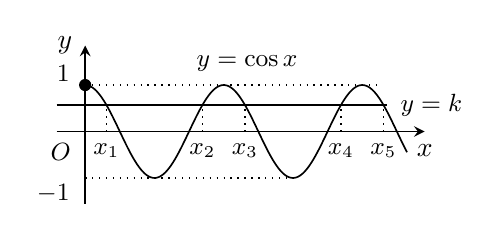
\begin{tikzpicture}[line width=0.6pt, x=0.28cm, y=0.59cm]
  \draw[dotted, line width=0.5pt] (0,1) -- (13.4,1);
  \draw[dotted, line width=0.5pt] (0,-1) -- (9.6,-1);
  \draw[->, >=stealth, line width=0.7pt] (-1.3,0) -- (15.4,0) node[below=1pt] {$x$};
  \draw[->, >=stealth, line width=0.7pt] (0,-1.55) -- (0,1.85) node[left=1pt] {$y$};
  \draw[line width=0.5pt] (-1.3,0.57) -- (13.7,0.57);
  \draw[domain=0:14.6, samples=220, smooth] plot (\x, {cos(57.2958*\x)});
  \draw[dotted, line width=0.5pt] (0.964,0) -- (0.964,0.57);
  \draw[dotted, line width=0.5pt] (5.319,0) -- (5.319,0.57);
  \draw[dotted, line width=0.5pt] (7.247,0) -- (7.247,0.57);
  \draw[dotted, line width=0.5pt] (11.602,0) -- (11.602,0.57);
  \draw[dotted, line width=0.5pt] (13.530,0) -- (13.530,0.57);
  \fill (0,1) circle (2.2pt);
  \node[anchor=south east, font=\small] at (-0.25,0.85) {$1$};
  \node[anchor=north east, font=\small] at (-0.25,-0.92) {$-1$};
  \node[anchor=north east, font=\small] at (-0.2,-0.05) {$\pt{O}$};
  \node[anchor=north, font=\small] at (0.964,-0.05) {$x_1$};
  \node[anchor=north, font=\small] at (5.319,-0.05) {$x_2$};
  \node[anchor=north, font=\small] at (7.247,-0.05) {$x_3$};
  \node[anchor=north, font=\small] at (11.602,-0.05) {$x_4$};
  \node[anchor=north, font=\small] at (13.530,-0.05) {$x_5$};
  \node[anchor=west, font=\small] at (13.85,0.57) {$y=k$};
  \node[anchor=south west, font=\small] at (4.6,1.08) {$y=\cos x$};
\end{tikzpicture}
}\end{center}
\dmchoicesauto{}{$24\pi$}{$26\pi$}{$28\pi$}{$30\pi$}{$32\pi$}
